\documentclass[]{article}

%opening
\title{Granger Causality note}
\author{Kate Nguyen}

\begin{document}

\maketitle

 \section{Granger Causality step-by-step}

Given two time series $X(t)$, $Y(t)$.

Hypothesis: $X(t)$ causes $Y(t)$.

We then construct restricted and unrestricted models:
\begin{align*}
	Y(t) &= \sum_{i = 1}^{k} \alpha_i Y(t-i)  + c_1 + \epsilon_t \hspace{5mm} \textbf{(Restricted)}\\
	Y(t) &= \sum_{i = 1}^{k} \alpha_i Y(t-i)  + \sum_{j = 1}^{k} \beta_j X(t-j) + c_2 + \epsilon_t^{'}  \hspace{5mm} \textbf{(Unrestricted)}
\end{align*}
where $\alpha_i$, $\beta_j$, $c_1$, $c_2$ are coefficients, $\epsilon_t$, $\epsilon_t^{'}$ are residuals, and $k$ is the order of regression. 

To find the optimal order, we compare the AIC/BIC for each order. For a linear regression with $n$ observations and $k$ parameters used to fit, AIC and BIC can be determined by
\begin{align}
	\text{AIC} &= n \cdot \ln \Bigg( \frac{\text{SSE}}{n} \Bigg) + 2 \cdot (k + 1) \\
	\text{BIC} &= n \cdot \ln \Bigg( \frac{\text{SSE}}{n} \Bigg) + \ln (n) \cdot (k + 1)
\end{align}
AIC/BIC can be negative. The order that yields the least AIC/BIC is the optimal order.

Coefficients $\alpha_i$ and $\beta_j$ can be determined by minimizing the residuals, i.e. $\text{argmin} (Y_t - \sum_{i = 1}^{k} \alpha_i Y(t-1)  - c_1)$. We say $X(t)$ Granger causes $Y(t)$ when there is an improvement in residuals, i.e. $\epsilon_t^{'} <  \epsilon_t$.

The standard measure of G causality in the literature is defined for univariate predictor and predictee variables X and Y, and is given by the natural logarithm of the ratio of the residual variance in the restricted regression of the unrestricted regression:
\begin{align}
	F_{X \rightarrow Y} = \ln \frac{\text{Var}(\epsilon_t)}{\text{Var}(\epsilon_t^{'})}
\end{align}

The Granger causality has the following properties: 

(1) For scalar X and Y it is possible both for Y to G-cause X and for X to G-cause Y, a feedback stochastic process.

(2) $F$ can never be negative.

(3) Statistical significance can be determined via F-statistic:
\begin{align}
	\mathcal{F} = \frac{\frac{\text{RSS}_\text{r} - \text{RSS}_\text{ur}}{m}}{\frac{\text{RSS}_\text{ur}}{T - 2m - 1}}
	\label{F_stats}
\end{align}
where $\text{RSS}_\text{r} = \sum_{t = m + 1}^T \epsilon_t^2$

$\underline{\text{Null hypothesis:}}$ $\beta_j = 0 \hspace{1mm} \forall j$, i.e., $X(t)$ does not Granger cause $Y(t)$.

$\underline{\text{Alternate hypothesis:}}$ at least one of the lags of $X$ is significant, i.e. $X(t)$ Granger causes $Y(t)$.

From F-statistics formula \ref{F_stats}, we can determine the p-value. If the p-value is less than 0.05 (for $95 \%$ confidence interval), we reject the null hypothesis. Therefore, $X(t)$ Granger causes $Y(t)$.

Granger Causality is not symmetric. $X(t)$ Granger causes $Y(t)$ does not mean $Y(t)$ Granger causes $X(t)$. We repeat same steps for the opposite direction.

%------------------------------------------------------
\section{Examples}
%------------------------------------------------------

%------------------------------------------------------
\subsection{Chickens, Eggs, and Causality, or Which Came First?}
%------------------------------------------------------

Thurman and Fisher examined annual U.S. time series from 1930 to 1983 of egg production and chicken population and perforemed  Granger causality tests using one to four lags.

\begin{figure}[H]
	\begin{center}
		%\hspace{5cm}
		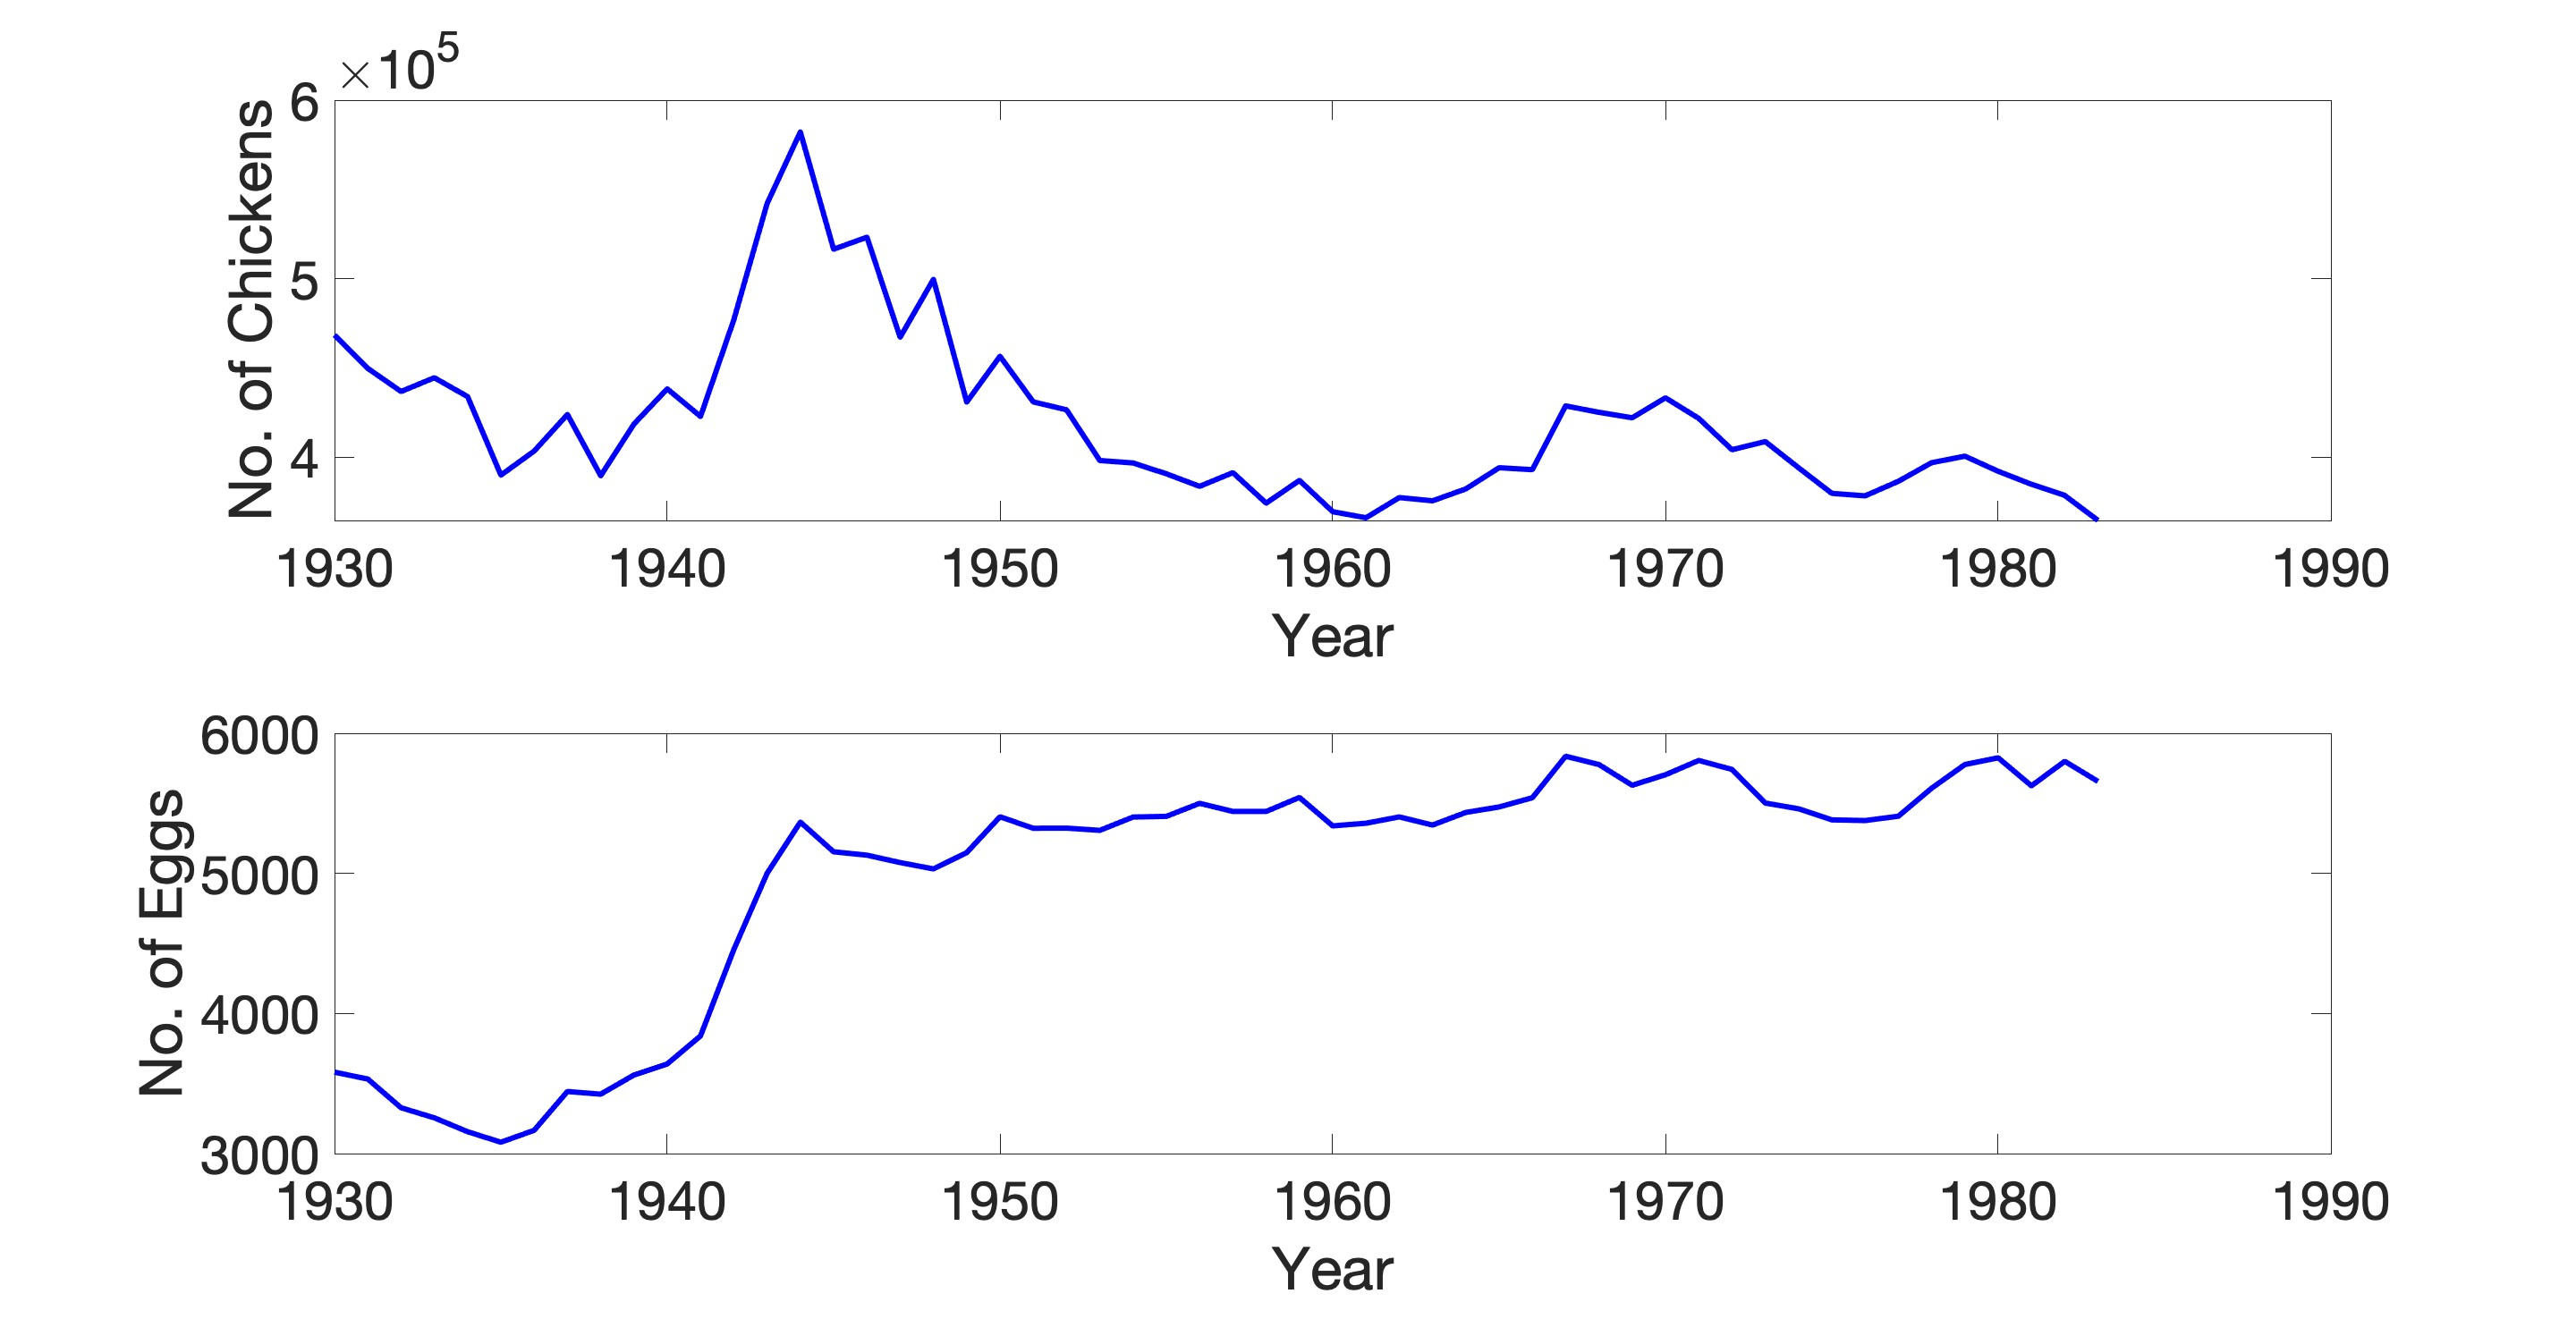
\includegraphics[width=15cm]{ChickenEgg_ts.jpg}
		\caption{Time series of chicken population (top) and egg production (bottom) from 1930 to 1983 in the United States. The data came from U.S. Department of Agriculture.}
		\label{ChickenEgg_ts} 
		\vspace{-4mm}
	\end{center}
\end{figure} 

To conclude that one ``came" first, they (1) reject the noncausality of the one to the other, and (2) at the same time fail to reject noncausality of the other to the one. If either both cause each other or neither causes the other, the question will remain unanswered.

First direction: did the chicken come first?
We considered the restricted and non-restricted linear regressions:
\begin{align}
	\text{Eggs}_t &= \sum_{i=1}^L \alpha_i \cdot \text{Eggs}_{t-1} + c + \epsilon_t  \label{Egg}
\end{align}
\begin{align}
	\text{Eggs}_t &= \sum_{i=1}^L \alpha_i \cdot \text{Eggs}_{t-1} + \sum_{i=1}^L \beta_i \cdot \text{Chickens}_{t-1} + c + \epsilon_t^{'} 
	\label{EggChicken}
\end{align}
where $L$ is number of lags, $c$ is constant, $\epsilon_t$ and $\epsilon_t^{'}$ are residuals of the linear regressions.


\begin{table}
	\begin{center}
		\begin{tabular}{ | c | c c c c c | c | }
			\hline
			Lags & $\alpha_1$ &  $\alpha_2$& $\alpha_3$ & $\alpha_4$ & $c$ & AIC  \\ \hline 
			1 & 0.9624 & N/A & N/A & N/A & 226.2566 & 546.3798 \\  \hline 
			2 & 1.3287 & -0.3725 & N/A & N/A & 243.7684 & 530.3606 \\  \hline
			3 & 1.3017 & -0.3608 & 0.0042 & N/A & 306.1473 & 519.7606 \\  \hline
			4 & 1.2677 & -0.3166 & -0.0402 & 0.0281 & 341.5484
			& 511.9186 \\  \hline
		\end{tabular}
		\caption{Table of coefficients for equation (\ref{Egg}). Lag 4 yields the least AIC, so 4 is optimal lag.}
	\end{center}
\end{table}

\begin{table}
	\begin{tabular}{ | c | c c c c c c c c c |}
		\hline
		L & $\alpha_1$ &  $\alpha_2$& $\alpha_3$ & $\alpha_4$ & $\beta_1$ &  $\beta_2$& $\beta_3$ & $\beta_4$  & $c$  \\ \hline 
		1 & 0.9624 & N/A & N/A & N/A & -0.0001 & N/A & N/A & N/A & 279.3413 \\  \hline 
		2 & 1.4414 & -0.4896 & N/A & N/A & -0.0013 & 0.0007 & N/A & N/A & 508.2338  \\  \hline 
		3 & 1.3892 & -0.4271 & -0.0221 & N/A & -0.0012 & 0.0010 & -0.0003 & N/A & 567.3588 \\  \hline 
		4 & 1.3697 & -0.4194 & 0.0744 & -0.0916 & -0.0012 & 0.0008 & -0.0005 & 0.0003 & 638.4819 \\  \hline 
	\end{tabular}
	\caption{Table of coefficients for equation (\ref{EggChicken}). The AIC for lags 1 to 4 are 548.3300, 532.4489, 523.7438, and 518.0381, respectively. Here, lag 4 yields the least AIC, so 4 is optimal lag.}
\end{table}

Finally, we compute the F-statistics (equation \ref{F_stats}) and p-value:
\begin{table}[H]
	\begin{center}
		\begin{tabular}{ | c | c | c |c | c | }
			\hline
			Lags & $m$ &  $T$& F statistics & p-value   \\ \hline 
			1 & 1 & 53 & 0.0470 & 0.8292  \\ \hline 
			2 & 2 & 52 & 0.8800 & 0.4215 \\ \hline 
			3 & 3 & 51 & 0.5916 & 0.6238 \\ \hline 
			4 & 4 & 50 & 0.3929 & 0.8125 \\ \hline 
		\end{tabular}
		\caption{Table of lags, degree of freedom $m$, total number of observations $T$, F statistics and p-value corresponding to those parameters to determine the statistical significance of chickens Granger causes eggs.}
		\label{CE_stats}
	\end{center}
\end{table}
Recall our null hypothesis and alternate hypothesis:

$H_0: \beta_1 = \beta_2 = \cdots = \beta_L = 0$ (chickens do not Granger cause eggs).

$H_A:$ At least one of $\beta$ is non-zero (chickens Granger cause eggs)

Table \ref{CE_stats} failed to reject our null hypothesis at $5 \%$ level.

Second direction: did the egg come first?
We considered the restricted and non-restricted linear regressions:
\begin{align}
	\text{Chickens}_t &= \sum_{i=1}^L \alpha_i \cdot \text{Chickens}_{t-1} + c + \epsilon_t  \label{Chicken}
\end{align}
\begin{align}
	\text{Chickens}_t &= \sum_{i=1}^L \alpha_i \cdot \text{Chickens}_{t-1} + \sum_{i=1}^L \beta_i \cdot \text{Eggs}_{t-1} + c + \epsilon_t^{'} 
	\label{ChickenEgg}
\end{align}
where $L$ is number of lags, $c$ is constant, $\epsilon_t$ and $\epsilon_t^{'}$ are residuals of the linear regressions.


\begin{table}
	\begin{center}
		\begin{tabular}{ | c | c c c c c | c | }
			\hline
			Lags & $\alpha_1$ &  $\alpha_2$& $\alpha_3$ & $\alpha_4$ & $c$ & AIC  \\ \hline 
			1 & 0.8500 & N/A & N/A & N/A & 6.1130e4 & 1,074.7 \\  \hline 
			2 & 0.7576 & 0.1141 & N/A & N/A & 5.1983e4 & 1,056.6 \\  \hline
			3 & 0.7838 & 0.3134 & -0.2567  & N/A & 6.5750e+04 & 1,035.8 \\  \hline
			4 & 0.7790 & 0.3266 & -0.2387 & -0.0384 & 7.0589e+04 & 1,018.1 \\  \hline
		\end{tabular}
		\caption{Table of coefficients for equation (\ref{Chicken}). Lag 4 yields the least AIC, so 4 is optimal lag.}
	\end{center}
\end{table}

\begin{table}
	\begin{tabular}{ | c | c c c c c c c c c |}
		\hline
		L & $\alpha_1$ &  $\alpha_2$& $\alpha_3$ & $\alpha_4$ & $\beta_1$ &  $\beta_2$& $\beta_3$ & $\beta_4$  & $c$  \\ \hline 
		1 & 0.8349 & N/A & N/A & N/A & -4.3214 & N/A & N/A & N/A & 8.8952e4 \\  \hline 
		2 & 0.3280 & 0.4646 & N/A & N/A & 89.2693 & -94.2842 & N/A & N/A & 1.0566e+05  \\  \hline 
		3 & 0.2920 & 0.4453 & 0.0041 & N/A & 76.5731 & -47.0783 & -35.9327 & N/A & 1.3354e5\\  \hline 
		4 & 0.2333& 0.4580 & -0.0185 & 0.0257 & 87.3847 & -62.4941 & -8.2145 & -22.6355 & 1.4733e+05 \\  \hline 
	\end{tabular}
	\caption{Table of coefficients for equation (\ref{ChickenEgg}). The AIC for lags 1 to 4 are 1.0754e3, 1.0441e3, 1.0258e3, and 1.0087e3, respectively. Here, lag 4 yields the least AIC, so 4 is optimal lag.}
\end{table}

We compute the F-statistics (equation \ref{F_stats}) and p-value:
\begin{table}[H]
	\begin{center}
		\begin{tabular}{ | c | c | c |c | c | }
			\hline
			Lags & $m$ &  $T$& F statistics & p-value   \\ \hline 
			1 & 1 & 53 & 1.2071 & 0.2772  \\ \hline 
			2 & 2 & 52 & 8.8175 & 0.0006 \\ \hline 
			3 & 3 & 51 & 5.40506 & 0.0030 \\ \hline 
			4 & 4 & 50 & 4.2568 & 0.0057 \\ \hline 
		\end{tabular}
		\caption{Table of lags, degree of freedom $m$, total number of observations $T$, F statistics and p-value corresponding to those parameters to determine the statistical significance of eggs Granger causes chickens.}
		\label{EC_stats}
	\end{center}
\end{table}

$H_0: \beta_1 = \beta_2 = \cdots = \beta_L = 0$ (eggs do not Granger cause chickens).

$H_A:$ At least one of $\beta$ is non-zero (eggs Granger cause chickens)

F-statistics and p-values obtained from table \ref{EC_stats} rejects the null hypothesis.

Therefore, we can conclude that eggs came first. This is the same conclusion as in Thurman's and Fisher's paper.



\end{document}
